\documentclass{beamer}
\usetheme{Singapore}
\usepackage[round,sort]{natbib}
\usepackage{tikz}
\usetikzlibrary{arrows,decorations.pathmorphing,backgrounds,fit,positioning,shapes.symbols,chains}
\usepackage{adjustbox}
\usepackage{verbatim}
\usepackage{graphicx}
\usepackage{hyperref}

\usepackage{tabu}
\hypersetup{
    colorlinks=true,
    linkcolor=blue,
    filecolor=cyan,      
    urlcolor=cyan,
    citecolor=blue,
}

\graphicspath{ {qe-paper-presentation-images/} }

\title{Heterogeneity in Knowledge Flows of Regions: Impact on Invention Quality}
%\subtitle{QE Research Paper}
\author{Ashwin Iyenggar}
\institute[Indian Institute of Management Bangalore] 
{
  Strategy Area\\
  Indian Institute of Management Bangalore
}
\date{22 June, 2017}
\subject{Heterogeneity in Knowledge Flows of Regions: Impact on Invention Quality}

% \pgfdeclareimage[height=0.5cm]{university-logo}{university-logo-filename}
% \logo{\pgfuseimage{university-logo}}

\AtBeginSubsection[]
{
  \begin{frame}<beamer>{Outline}
    \tableofcontents[currentsection,currentsubsection]
  \end{frame}
}

\begin{document}

\begin{frame}
  \titlepage
\end{frame}

\begin{frame}{Outline}
  \tableofcontents
  % You might wish to add the option [pausesections]
\end{frame}


\section{Motivation}
\begin{frame}{Research Question}{}
\begin{itemize}
\item{}
\end{itemize}
\end{frame}

\section{Literature Review}

\section{Theory}
\begin{frame}{Hypotheses}{}
Create four slides and on each put up in pictures the various mechanisms and effects that literature suggests
\end{frame}



\section{Data and Method}
\begin{frame}{Geographic Mapping}{San Jose}
\begin{figure}[h!]
\begin{centering}
  \includegraphics[width=0.6\textwidth]{SanJose}
  \caption{Geographic Definition of San Jose, CA}
   \label{fig:SanJose}
\end{centering}
\end{figure}
\end{frame}


\begin{frame}{Methodology}{}
\begin{itemize}
\item{Data Source: Patents from USPTO, source: patentsview.org}
\item{Data Source: Regions using Remote Sensing Data, source: naturalearthdata.com}
\item{Unit of Analysis: Region-Year}
\item{Dependent Variables: Total Citations Received, Non-Self Citations Received}
\item{Independent Variables: Share of citations made within/outside region, within/outside assignee}
\item{Control Variables: Technology subcategories \citep*{Hall2001a}, Region fixed effects, Year effects}
\item{Estimation Method: Negative Binomial}
\end{itemize}
\end{frame}

\begin{frame}{Addressing Potential Issues}{}
\begin{itemize}
\item{Dir}
\end{itemize}
\end{frame}

\begin{frame}{Results}{}

\end{frame}

\section{Future Work}
\begin{frame}{Limitations and Future Work}{}
\begin{itemize}
\item{C}

\end{itemize}
\end{frame}

\bibliography{/Users/aiyenggar/code/bibliography/aiyenggar}
\bibliographystyle{ai-amjlike}

\end{document}

\begin{comment}

\begin{frame}{Geographic Mapping}{Bangalore}
\begin{figure}[h!]
\begin{centering}
  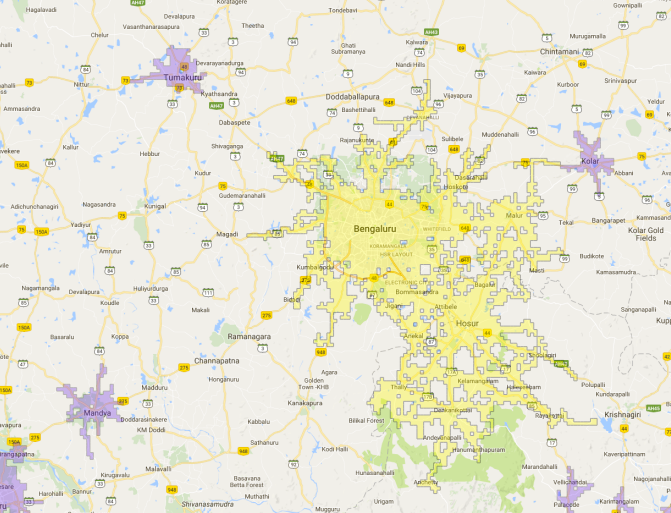
\includegraphics[width=0.7\textwidth]{Bangalore}
  \caption{Geographic Definition of Bangalore}
   \label{fig:Bangalore}
\end{centering}
\end{figure}
\end{frame}


\begin{figure}[h]
\begin{centering}
  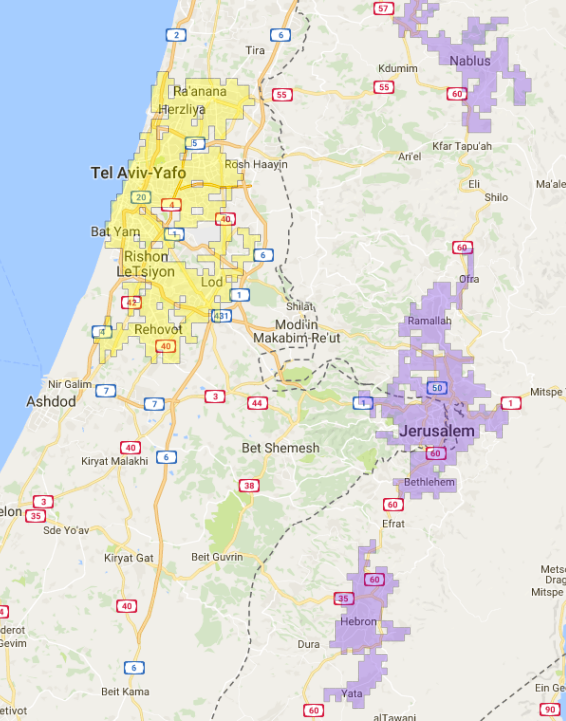
\includegraphics[width=\textwidth]{TelAviv}
  \caption{Geographic Definition of Tel Aviv-Yafo}
   \label{fig:TelAviv}
\end{centering}
\end{figure}
\end{comment}

